\PassOptionsToPackage{unicode=true}{hyperref} % options for packages loaded elsewhere
\PassOptionsToPackage{hyphens}{url}
%
\documentclass[ignorenonframetext,]{beamer}
\setbeamertemplate{caption}[numbered]
\setbeamertemplate{caption label separator}{: }
\setbeamercolor{caption name}{fg=normal text.fg}
\beamertemplatenavigationsymbolsempty
\usepackage{lmodern}
\usepackage{amssymb,amsmath}
\usepackage{ifxetex,ifluatex}
\usepackage{fixltx2e} % provides \textsubscript
\ifnum 0\ifxetex 1\fi\ifluatex 1\fi=0 % if pdftex
  \usepackage[T1]{fontenc}
  \usepackage[utf8]{inputenc}
  \usepackage{textcomp} % provides euro and other symbols
\else % if luatex or xelatex
  \usepackage{unicode-math}
  \defaultfontfeatures{Ligatures=TeX,Scale=MatchLowercase}
\fi
\usetheme[]{metropolis}
% use upquote if available, for straight quotes in verbatim environments
\IfFileExists{upquote.sty}{\usepackage{upquote}}{}
% use microtype if available
\IfFileExists{microtype.sty}{%
\usepackage[]{microtype}
\UseMicrotypeSet[protrusion]{basicmath} % disable protrusion for tt fonts
}{}
\IfFileExists{parskip.sty}{%
\usepackage{parskip}
}{% else
\setlength{\parindent}{0pt}
\setlength{\parskip}{6pt plus 2pt minus 1pt}
}
\usepackage{hyperref}
\hypersetup{
            pdftitle={StatCafe},
            pdfauthor={Eli Kravitz},
            pdfborder={0 0 0},
            breaklinks=true}
\urlstyle{same}  % don't use monospace font for urls
\newif\ifbibliography
\usepackage{color}
\usepackage{fancyvrb}
\newcommand{\VerbBar}{|}
\newcommand{\VERB}{\Verb[commandchars=\\\{\}]}
\DefineVerbatimEnvironment{Highlighting}{Verbatim}{commandchars=\\\{\}}
% Add ',fontsize=\small' for more characters per line
\usepackage{framed}
\definecolor{shadecolor}{RGB}{248,248,248}
\newenvironment{Shaded}{\begin{snugshade}}{\end{snugshade}}
\newcommand{\AlertTok}[1]{\textcolor[rgb]{0.94,0.16,0.16}{#1}}
\newcommand{\AnnotationTok}[1]{\textcolor[rgb]{0.56,0.35,0.01}{\textbf{\textit{#1}}}}
\newcommand{\AttributeTok}[1]{\textcolor[rgb]{0.77,0.63,0.00}{#1}}
\newcommand{\BaseNTok}[1]{\textcolor[rgb]{0.00,0.00,0.81}{#1}}
\newcommand{\BuiltInTok}[1]{#1}
\newcommand{\CharTok}[1]{\textcolor[rgb]{0.31,0.60,0.02}{#1}}
\newcommand{\CommentTok}[1]{\textcolor[rgb]{0.56,0.35,0.01}{\textit{#1}}}
\newcommand{\CommentVarTok}[1]{\textcolor[rgb]{0.56,0.35,0.01}{\textbf{\textit{#1}}}}
\newcommand{\ConstantTok}[1]{\textcolor[rgb]{0.00,0.00,0.00}{#1}}
\newcommand{\ControlFlowTok}[1]{\textcolor[rgb]{0.13,0.29,0.53}{\textbf{#1}}}
\newcommand{\DataTypeTok}[1]{\textcolor[rgb]{0.13,0.29,0.53}{#1}}
\newcommand{\DecValTok}[1]{\textcolor[rgb]{0.00,0.00,0.81}{#1}}
\newcommand{\DocumentationTok}[1]{\textcolor[rgb]{0.56,0.35,0.01}{\textbf{\textit{#1}}}}
\newcommand{\ErrorTok}[1]{\textcolor[rgb]{0.64,0.00,0.00}{\textbf{#1}}}
\newcommand{\ExtensionTok}[1]{#1}
\newcommand{\FloatTok}[1]{\textcolor[rgb]{0.00,0.00,0.81}{#1}}
\newcommand{\FunctionTok}[1]{\textcolor[rgb]{0.00,0.00,0.00}{#1}}
\newcommand{\ImportTok}[1]{#1}
\newcommand{\InformationTok}[1]{\textcolor[rgb]{0.56,0.35,0.01}{\textbf{\textit{#1}}}}
\newcommand{\KeywordTok}[1]{\textcolor[rgb]{0.13,0.29,0.53}{\textbf{#1}}}
\newcommand{\NormalTok}[1]{#1}
\newcommand{\OperatorTok}[1]{\textcolor[rgb]{0.81,0.36,0.00}{\textbf{#1}}}
\newcommand{\OtherTok}[1]{\textcolor[rgb]{0.56,0.35,0.01}{#1}}
\newcommand{\PreprocessorTok}[1]{\textcolor[rgb]{0.56,0.35,0.01}{\textit{#1}}}
\newcommand{\RegionMarkerTok}[1]{#1}
\newcommand{\SpecialCharTok}[1]{\textcolor[rgb]{0.00,0.00,0.00}{#1}}
\newcommand{\SpecialStringTok}[1]{\textcolor[rgb]{0.31,0.60,0.02}{#1}}
\newcommand{\StringTok}[1]{\textcolor[rgb]{0.31,0.60,0.02}{#1}}
\newcommand{\VariableTok}[1]{\textcolor[rgb]{0.00,0.00,0.00}{#1}}
\newcommand{\VerbatimStringTok}[1]{\textcolor[rgb]{0.31,0.60,0.02}{#1}}
\newcommand{\WarningTok}[1]{\textcolor[rgb]{0.56,0.35,0.01}{\textbf{\textit{#1}}}}
% Prevent slide breaks in the middle of a paragraph:
\widowpenalties 1 10000
\raggedbottom
\setbeamertemplate{part page}{
\centering
\begin{beamercolorbox}[sep=16pt,center]{part title}
  \usebeamerfont{part title}\insertpart\par
\end{beamercolorbox}
}
\setbeamertemplate{section page}{
\centering
\begin{beamercolorbox}[sep=12pt,center]{part title}
  \usebeamerfont{section title}\insertsection\par
\end{beamercolorbox}
}
\setbeamertemplate{subsection page}{
\centering
\begin{beamercolorbox}[sep=8pt,center]{part title}
  \usebeamerfont{subsection title}\insertsubsection\par
\end{beamercolorbox}
}
\AtBeginPart{
  \frame{\partpage}
}
\AtBeginSection{
  \ifbibliography
  \else
    \frame{\sectionpage}
  \fi
}
\AtBeginSubsection{
  \frame{\subsectionpage}
}
\setlength{\emergencystretch}{3em}  % prevent overfull lines
\providecommand{\tightlist}{%
  \setlength{\itemsep}{0pt}\setlength{\parskip}{0pt}}
\setcounter{secnumdepth}{0}

% set default figure placement to htbp
\makeatletter
\def\fps@figure{htbp}
\makeatother

\usepackage{verbatim,color,amssymb,bbm,epsfig}
\usepackage{fancyhdr}
\usepackage[authoryear, sort]{natbib}
\usepackage{graphicx}
\usepackage{float}
 


%\usepackage[inline]{showlabels}

%\newcommand{\ind}{\mathbbm{1}}
%$\ind$



\newtheorem{Thm}{\underline{\bf Theorem}}
\newtheorem{Assume}{\underline{\bf Assumptions}}
\newtheorem{Mth}{Main Theorem}
\newtheorem{Def}{Definition}
\newtheorem{Rem}{\underline{\bf Remark}}
\newtheorem{Qes}{Question}
\newtheorem{proposition}{Proposition}
\newtheorem{Lem}{\underline{\bf Lemma}}
\newtheorem{Cor}{\underline{\bf Corollary}}
\newtheorem{Exa}{Example}
\newtheorem{Eq}{Equation}
\newtheorem{Alg}{Algorithm}
\def\rest{\hbox{rest}}

\newcommand{\MyProof}{\noindent\textbf{Proof. }}



\def\nN{\mathbb{N}}
\def\rR{\mathbb{R}}
\def\eE{\mathbb{E}}
\def\Supp{Supplementary Material}

\def\L{{\cal L}}
\def\B{\oldboldbeta}
\def\C{{\cal C}}
\def\D{{\cal D}}
\def\E{{\cal E}}
\def\F{{\cal F}}
\def\G{{\cal G}}
\def\K{{\cal K}}

\def\T{{\cal T}}
\def\U{{\cal U}}
\def\W{{\cal W}}
\def\V{{\cal V}}
\def\X{{\cal X}}
\def\Z{{\cal Z}}
\def\Y{{\cal Y}}
\def\boxit#1{\vbox{\hrule\hbox{\vrule\kern6pt  \vbox{\kern6pt#1\kern6pt}\kern6pt\vrule}\hrule}}
\def\rjccomment#1{\vskip 2mm\boxit{\vskip 2mm{\color{black}\bf#1} {\color{blue}\bf -- RJC\vskip 2mm}}\vskip 2mm}
\def\DRcomment#1{\vskip 2mm\boxit{\vskip 2mm{\color{black}\bf#1} {\color{blue}\bf -- DR\vskip 2mm}}\vskip 2mm}

\def\EKcomment#1{\vskip 2mm\boxit{\vskip 2mm{\color{black}\bf#1} {\color{blue}\bf -- Eli\vskip 2mm}}\vskip 2mm}

\def\wt{\widetilde}
\def\sumi{\hbox{$\sum_{i=1}^n$}}
\def\sumj{\hbox{$\sum_{j=1}^J$}}
\def\sumk{\hbox{$\sum_{k=1}^K$}}
\def\diag{\hbox{diag}}
\def\wh{\widehat}
\def\AIC{\hbox{AIC}}
\def\BIC{\hbox{BIC}}
\def\diag{\hbox{diag}}
\def\log{\hbox{log}}
\def\bias{\hbox{bias}}
\def\Siuu{\boldSigma_{i,uu}}
\def\ANNALS{{\it Annals of Statistics}}
\def\BIOK{{\it Biometrika}}
\def\whT{\widehat{\Theta}}
\def\STATMED{{\it Statistics in Medicine}}
\def\STATSCI{{\it Statistical Science}}
\def\JSPI{{\it Journal of Statistical Planning \& Inference}}
\def\JRSSB{{\it Journal of the Royal Statistical Society, Series B}}
\def\BMCS{{\it Biometrics}}
\def\COMMS{{\it Communications in Statistics, Theory \& Methods}}
\def\JQT{{\it Journal of Quality Technology}}
\def\STIM{{\it Statistics in Medicine}}
\def\TECH{{\it Technometrics}}
\def\AJE{{\it American Journal of Epidemiology}}
\def\JASA{{\it Journal of the American Statistical Association}}
\def\CDA{{\it Computational Statistics \& Data Analysis}}
\def\JCGS{{\it Journal of Computational and Graphical Statistics}}
\def\JCB{{\it Journal of Computational Biology}}
\def\BIOINF{{\it Bioinformatics}}
\def\JAMA{{\it Journal of the American Medical Association}}
\def\JNUTR{{\it Journal of Nutrition}}
\def\JCGS{{\it Journal of Computational and Graphical Statistics}}
\def\LETTERS{{\it Letters in Probability and Statistics}}
\def\JABES{{\it Journal of Agricultural, Biological and
                      Environmental Statistics}}
\def\JASA{{\it Journal of the American Statistical Association}}
\def\ANNALS{{\it Annals of Statistics}}
\def\JSPI{{\it Journal of Statistical Planning \& Inference}}
\def\TECH{{\it Technometrics}}
\def\BIOK{{\it Bio\-me\-tri\-ka}}
\def\JRSSB{{\it Journal of the Royal Statistical Society, Series B}}
\def\BMCS{{\it Biometrics}}
\def\COMMS{{\it Communications in Statistics, Series A}}
\def\JQT{{\it Journal of Quality Technology}}
\def\SCAN{{\it Scandinavian Journal of Statistics}}
\def\AJE{{\it American Journal of Epidemiology}}
\def\STIM{{\it Statistics in Medicine}}
\def\ANNALS{{\it Annals of Statistics}}
\def\whT{\widehat{\Theta}}
\def\STATMED{{\it Statistics in Medicine}}
\def\STATSCI{{\it Statistical Science}}
\def\JSPI{{\it Journal of Statistical Planning \& Inference}}
\def\JRSSB{{\it Journal of the Royal Statistical Society, Series B}}
\def\BMCS{{\it Biometrics}}
\def\COMMS{{\it Communications in Statistics, Theory \& Methods}}
\def\JQT{{\it Journal of Quality Technology}}
\def\STIM{{\it Statistics in Medicine}}
\def\TECH{{\it Technometrics}}
\def\AJE{{\it American Journal of Epidemiology}}
\def\JASA{{\it Journal of the American Statistical Association}}
\def\CDA{{\it Computational Statistics \& Data Analysis}}
\def\dfrac#1#2{{\displaystyle{#1\over#2}}}
\def\VS{{\vskip 3mm\noindent}}
\def\refhg{\hangindent=20pt\hangafter=1}
\def\refmark{\par\vskip 2mm\noindent\refhg}
\def\naive{\hbox{naive}}
\def\itemitem{\par\indent \hangindent2\parindent \textindent}
\def\var{\hbox{var}}
\def\cov{\hbox{cov}}
\def\corr{\hbox{corr}}
\def\trace{\hbox{trace}}
\def\refhg{\hangindent=20pt\hangafter=1}
\def\refmark{\par\vskip 2mm\noindent\refhg}
\def\Normal{\hbox{Normal}}
\def\povr{\buildrel p\over\longrightarrow}
\def\ccdot{{\bullet}}
\def\bse{\begin{eqnarray*}}
\def\ese{\end{eqnarray*}}
\def\be{\begin{eqnarray}}
\def\ee{\end{eqnarray}}
\def\bq{\begin{equation}}
\def\eq{\end{equation}}
\def\bse{\begin{eqnarray*}}
\def\ese{\end{eqnarray*}}
\def\pr{\hbox{pr}}
\def\wh{\widehat}
\def\trans{^{\rm T}}
\def\myalpha{{\cal A}}
\def\th{^{th}}
\def\b1e{{\mathbf e}}
\def\bx{{\mathbf x}}
\def\bX{{\mathbf X}}
\def\B{{\mathbf B}}
\def\C{{\mathbf C}}
\def\bw{{\mathbf w}}
\def\bS{{\mathbf S}}
\def\bzero{{\mathbf 0}}
\newcommand{\etam}{\mbox{\boldmath $\eta$}}
\newcommand{\bbeta}{\mbox{\boldmath $\beta$}}
\newcommand{\bgamma}{\mbox{\boldmath $\gamma$}}
\newcommand{\bzeta}{\mbox{\boldmath $\zeta$}}
\newcommand{\bSigma}{\mbox{\boldmath $\Sigma$}}
\newcommand{\balpha}{\mbox{\boldmath $\alpha$}}
\newcommand{\bomega}{\mbox{\boldmath $\omega$}}
\def\bW{\W}


\def\bfa{{\bf a}}
\def\bfA{{\bf A}}
\def\bfb{{\bf b}}
\def\bfB{{\bf B}}
\def\bfc{{\bf c}}
\def\bfC{{\bf C}}
\def\bfd{{\bf d}}
\def\bfD{{\bf D}}
\def\bfe{{\bf e}}
\def\bfE{{\bf E}}
\def\bff{{\bf f}}
\def\bfF{{\bf F}}
\def\bfg{{\bf g}}
\def\bfG{{\bf G}}
\def\bfh{{\bf h}}
\def\bfH{{\bf H}}
\def\bfi{{\bf i}}
\def\bfI{{\bf I}}
\def\bfj{{\bf j}}
\def\bfJ{{\bf J}}
\def\bfk{{\bf k}}
\def\bfK{{\bf K}}
\def\bfl{{\bf l}}
\def\bfL{{\bf L}}
\def\bfm{{\bf m}}
\def\bfM{{\bf M}}
\def\bfn{{\bf n}}
\def\bfN{{\bf N}}
\def\bfo{{\bf o}}
\def\bfO{{\bf O}}
\def\bfp{{\bf p}}
\def\bfP{{\bf P}}
\def\bfq{{\bf q}}
\def\bfQ{{\bf Q}}
\def\bfr{{\bf r}}
\def\bfR{{\bf R}}
\def\bfs{{\bf s}}
\def\bfS{{\bf S}}
\def\bft{{\bf t}}
\def\bfT{{\bf T}}
\def\bfu{{\bf u}}
\def\bfU{{\bf U}}
\def\bfv{{\bf v}}
\def\bfV{{\bf V}}
\def\bfw{{\bf w}}
\def\bfW{{\bf W}}
\def\bfx{{\bf x}}
\def\bfX{{\bf X}}
\def\bfy{{\bf y}}
\def\bfY{{\bf Y}}
\def\bfz{{\bf z}}
\def\bfZ{{\bf Z}}
\def\boldalpha{\boldmath\alpha}
\def\boldAlpha{\boldmath\Alpha}
\def\boldbeta{\boldmath\beta}
\def\boldBeta{\boldmath\beta}
\def\bolddelta{\boldmath\delta}
\def\boldDelta{\boldmath\Delta}
\def\boldeta{\boldmath\eta}
\def\boldEta{\boldmath\Eta}
\def\boldgamma{\boldmath\gamma}
\def\boldGamma{\boldmath\Gamma}
\def\boldlambda{\boldmath\lambda}
\def\boldLambda{\boldmath\Lambda}
\def\boldmu{\boldmath\mu}
\def\boldMu{\boldmath\Mu}
\def\boldnu{\boldmath\nu}
\def\boldNu{\boldmath\Nu}
\def\boldomega{\boldmath\omega}
\def\boldOmega{\boldmath\Omega}
\def\boldpsi{\boldmath\psi}
\def\boldPsi{\boldmath\Psi}
\def\boldsigma{\boldmath\sigma}
\def\boldSigma{\boldmath\Sigma}
\def\boldpi{\boldmath\pi}
\def\boldPi{\boldmath\Pi}
\def\boldphi{\boldmath\phi}
\def\boldepsilon{\boldmath\epsilon}
\def\boldtheta{\boldmath\theta}
\def\boldTheta{\boldmath\Theta}
\def\boldve{\boldmath\ve}
\def\boldVe{\boldmath\Epsilon}
\def\boldxi{\boldmath\xi}
\def\boldXi{\boldmath\Omega}
\def\boldzeta{\boldmath\zeta}
\def\boldZeta{\boldmath\Zeta}
\def\trans{^{\rm T}}
\def\myalpha{{\cal A}}
\def\th{^{th}}
\def\b1e{{\mathbf e}}
\def\bB{{\mathbf B}}
\def\bc{{\mathbf c}}
\def\bC{{\mathbf C}}
\def\bp{{\mathbf p}}
\def\bu{{\mathbf u}}
\def\bU{{\mathbf U}}
\def\bw{{\mathbf w}}
\def\bW{{\mathbf W}}
\def\bx{{\mathbf x}}
\def\bX{{\mathbf X}}
\def\by{{\mathbf y}}
\def\bY{{\mathbf Y}}
\def\bz{{\mathbf z}}
\def\bZ{{\mathbf Z}}
\def\bS{{\mathbf S}}
\def\bzero{{\mathbf 0}}

\def\whT{\widehat{\Theta}}
\def\te{\widetilde{e}}
\def\te{\widetilde{\epsilon}}
\def\tp{\widetilde{p}}
\def\tv{\widetilde{v}}
\def\tmu{\widetilde{\mu}}
\def\tsigma{\widetilde{\sigma}}
\def\sumb{\hbox{$\sum_{b=1}^{B}$}}


\def\colblue#1{\textcolor{blue}{#1}}
\def\highlight#1{\underline{\textcolor{red}{#1}}}
\def\boxit#1{\vbox{\hrule\hbox{\vrule\kern6pt \vbox{\kern6pt \textcolor{blue}{#1}\kern6pt}\kern6pt\vrule}\hrule}}
\def\rjccomment#1{\vskip 2mm\boxit{\vskip 2mm{\color{black}\bf#1} {\color{blue}\bf -- RJC\vskip 2mm}}\vskip 2mm}
\def\ascomment#1{\vskip 2mm\boxit{\vskip 2mm{\color{blue}\bf#1} {\color{black}\bf -- Abhra\vskip 2mm}}\vskip 2mm}

\def\authorfootnote#1{{\let\thefootnote\relax\footnotetext{#1}}}
\def\scar{{\color{red}\bf {\tt scar}}}
\def\K{{\cal K}}

\setbeamercolor{alerted text}{fg=blue}
\setbeamerfont{alerted text}{series=\bfseries}

\title{StatCafe}
\author{Eli Kravitz}
\date{2/28/2019}

\begin{document}
\frame{\titlepage}

\begin{frame}{Introduction}
\protect\hypertarget{introduction}{}

\begin{itemize}
\item
  I will give an \alert{opinionated} way for you to manage your research
  workflow in R.

  \begin{itemize}
  \tightlist
  \item
    I’ve learned this through trial and error\ldots{} mostly error.
  \end{itemize}
\item
  Take parts of this you like, ignore parts you don’t
\item
  Many people are more qualified to talk about this

  \begin{itemize}
  \tightlist
  \item
    none of them will come here and do it for free. You’re stuck with me
  \end{itemize}
\end{itemize}

\end{frame}

\begin{frame}{Scenarios (totally not based on personal experience)}
\protect\hypertarget{scenarios-totally-not-based-on-personal-experience}{}

\begin{itemize}
\item
  \textbf{Scenarios 1}: You work on a project, complete 90\% of it, then
  stop working on it for 2 years.

  \begin{itemize}
  \tightlist
  \item
    \alert{Nothing works} on your new computer, you can’t locate all the
    data and files you need.
  \end{itemize}
\item
  \textbf{Scenarios 2}: You have a simulation working perfectly. You
  make a lot of changes. \alert{A few days later} you can’t remember why
  you made these changes, and now
  \alert{your simulation does not work correctly}.
\item
  \textbf{Scenarios 3}: You decide to rewrite most of the paper, show it
  to your advisor, and they tell you it was better before.

  \begin{itemize}
  \tightlist
  \item
    You only have the old draft of the paper in PDF. You DO NOT want to
    retype it.
  \end{itemize}
\end{itemize}

\end{frame}

\begin{frame}{Storing Everything: Rprojects}
\protect\hypertarget{storing-everything-rprojects}{}

\begin{itemize}
\item
  I organize all my research projects the same way.

  \begin{itemize}
  \tightlist
  \item
    Show folder structure
  \end{itemize}
\item
  Make the directory a Rproject.
\item
  R projects let you:

  \begin{itemize}
  \tightlist
  \item
    Divide your work naturally
  \item
    Store environments for every project
  \item
    “freeze” R in a state that works (advanced, won’t cover)
  \end{itemize}
\item
  Integrates nicely other things we’ll cover
\end{itemize}

\end{frame}

\begin{frame}{Making an R project}
\protect\hypertarget{making-an-r-project}{}

\begin{itemize}
\tightlist
\item
  Go to File \(\rightarrow\) New Project
\end{itemize}

\begin{center}
  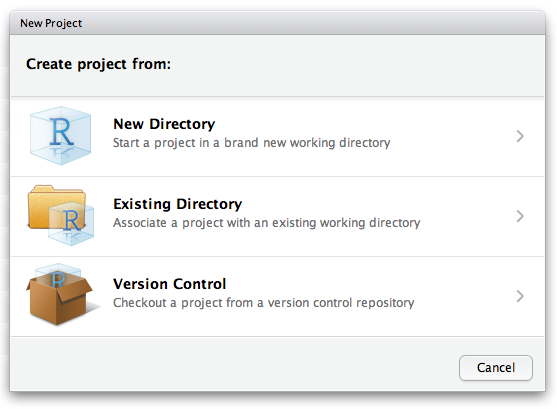
\includegraphics[width=\textwidth,height= .90\textheight,keepaspectratio]{projects_new.png}
\end{center}

\end{frame}

\begin{frame}{Making an R project}
\protect\hypertarget{making-an-r-project-1}{}

\begin{itemize}
\item
  Follow the prompts to make your project.
\item
  You’re done. Easy.
\item
  Now do this \alert{every time} you start a new research project.
\end{itemize}

\end{frame}

\begin{frame}[fragile]{Relative Filepaths and here()}
\protect\hypertarget{relative-filepaths-and-here}{}

\begin{itemize}
\tightlist
\item
  Does your R code start with this?
\end{itemize}

\begin{Shaded}
\begin{Highlighting}[]
\KeywordTok{setwd}\NormalTok{(}\StringTok{"C:\textbackslash{}Users\textbackslash{}Eli\textbackslash{}path}\CharTok{\textbackslash{}t}\StringTok{hat\textbackslash{}only\textbackslash{}I\textbackslash{}have"}\NormalTok{)}
\NormalTok{mydata =}\StringTok{ }\KeywordTok{read.csv}\NormalTok{(data.csv)}
\end{Highlighting}
\end{Shaded}

\begin{itemize}
\item
  This is \alert{bad}. As soon as you rename or move directories, it
  breaks.
\item
  What if someone else wants to use your code? What if you want to use a
  different computer?
\end{itemize}

\end{frame}

\begin{frame}[fragile]{Relative Filepaths and here()}
\protect\hypertarget{relative-filepaths-and-here-1}{}

\begin{itemize}
\tightlist
\item
  Putting your files in an Rproject already helps. The directory is to
  to where the .Rproj file is.
\end{itemize}

\begin{Shaded}
\begin{Highlighting}[]
\KeywordTok{getwd}\NormalTok{()}
\end{Highlighting}
\end{Shaded}

\begin{verbatim}
## [1] "/Users/kravitze/Documents/SafeCafe/Code"
\end{verbatim}

\begin{itemize}
\tightlist
\item
  Let’s do better with the here package.
\end{itemize}

\end{frame}

\begin{frame}[fragile]{Relative Filepaths and here()}
\protect\hypertarget{relative-filepaths-and-here-2}{}

\begin{itemize}
\tightlist
\item
  Here looks for a .Rproj file and makes file paths relative
\end{itemize}

\begin{Shaded}
\begin{Highlighting}[]
\KeywordTok{here}\NormalTok{()}
\end{Highlighting}
\end{Shaded}

\begin{verbatim}
## [1] "/Users/kravitze/Documents/SafeCafe"
\end{verbatim}

\begin{Shaded}
\begin{Highlighting}[]
\KeywordTok{here}\NormalTok{(}\StringTok{"Inner_Directory"}\NormalTok{)}
\end{Highlighting}
\end{Shaded}

\begin{verbatim}
## [1] "/Users/kravitze/Documents/SafeCafe/Inner_Directory"
\end{verbatim}

\begin{itemize}
\item
  Code won’t need to change between computers
\item
  Example: Load data
\end{itemize}

\begin{Shaded}
\begin{Highlighting}[]
\NormalTok{my_data =}\StringTok{ }\KeywordTok{here}\NormalTok{(}\StringTok{"Data"}\NormalTok{, }\StringTok{"my_file.csv"}\NormalTok{)}
\end{Highlighting}
\end{Shaded}

\end{frame}

\begin{frame}{Saving Progress with Github}
\protect\hypertarget{saving-progress-with-github}{}

\begin{itemize}
\item
  Now nothing is tied to the filepaths on our computer.
\item
  How can we \alert{back everything up} and
  \alert{make it available on multiple computers}?
\item
  Github!
\end{itemize}

\end{frame}

\begin{frame}{Saving Progress with Github}
\protect\hypertarget{saving-progress-with-github-1}{}

\begin{itemize}
\tightlist
\item
  Setting up Github is simple, but many steps.

  \begin{itemize}
  \tightlist
  \item
    See links at the end for instructions
  \end{itemize}
\item
  I will go over what it can do for you, and why you should work with
  it.
\end{itemize}

\end{frame}

\begin{frame}{Saving Progress with Github}
\protect\hypertarget{saving-progress-with-github-2}{}

\begin{itemize}
\item
  Github let’s you track versions on your file
\item
  Github saves the history of your file
\item
  Made changes to your code \(\rightarrow\) you can
  \alert{revert back to an earlier}. version.
\item
  Works with .tex too!
\end{itemize}

\end{frame}

\end{document}
